% ============================================================
% JATIT Article - Full Improved Version (~16 pages)
% Advancing Heart Disease Diagnosis and ECG Classification
% Using Deep Learning and Explainable AI
% ============================================================
\documentclass[10pt, twocolumn]{article}

\usepackage[T1]{fontenc}
\usepackage[utf8]{inputenc}
\usepackage[english]{babel}
\usepackage{geometry}
\usepackage{amsmath, amssymb, amsfonts}
\usepackage{graphicx}
\usepackage{booktabs}
\usepackage{array}
\usepackage{multirow}
\usepackage{hyperref}
\usepackage{cite}
\usepackage{xcolor}
\usepackage{fancyhdr}
\usepackage{titlesec}
\usepackage{caption}
\usepackage{subcaption}
\usepackage{enumitem}
\usepackage[protrusion=true,expansion=false,babel=true]{microtype}
\usepackage{float}
\usepackage{parskip}

% --- Page geometry (JATIT style) ---
\geometry{
  a4paper,
  top=2.2cm, bottom=2.5cm,
  left=1.8cm, right=1.8cm,
  headheight=14pt
}

\graphicspath{{figures/}}
\setlength{\columnsep}{0.65cm}
\setlength{\parindent}{0pt}
\setlength{\parskip}{4pt}

% --- Header/Footer ---
\pagestyle{fancy}
\fancyhf{}
\renewcommand{\headrulewidth}{0.4pt}
\renewcommand{\footrulewidth}{0.4pt}
\fancyhead[L]{\footnotesize\textit{Journal of Theoretical and Applied Information Technology}}
\fancyhead[R]{\footnotesize\textit{31\textsuperscript{st} March 2026. Vol.104. No 6}}
\fancyfoot[L]{\footnotesize\textcopyright\ Little Lion Scientific}
\fancyfoot[C]{\footnotesize\textit{www.jatit.org}}
\fancyfoot[R]{\footnotesize\thepage}

% --- Section formatting ---
\titleformat{\section}{\normalsize\bfseries\MakeUppercase}{{\thesection.}}{0.5em}{}
\titleformat{\subsection}{\normalsize\bfseries}{{\thesubsection}}{0.5em}{}
\titleformat{\subsubsection}{\normalsize\itshape\bfseries}{{\thesubsubsection}}{0.5em}{}

% --- Hyperref ---
\hypersetup{colorlinks=true, linkcolor=blue, citecolor=blue, urlcolor=blue,
            pdftitle={Advancing Heart Disease Diagnosis Using Deep Learning and XAI},
            pdfauthor={Telmoud, Saleck, Tourad}}

% ─── Custom commands ──────────────────────────────────────────────────────────
\newcommand{\jatitline}{\noindent\rule{\linewidth}{0.4pt}\par}

% ============================================================
\begin{document}
% Global tolerance settings to suppress Underfull/Overfull hbox warnings
\sloppy
\emergencystretch=3em

% ─── TITLE BLOCK (one-column) ────────────────────────────────────────────────
\twocolumn[{%
\begin{center}
  \footnotesize
  ISSN: 1992-8645 \hfill E-ISSN: 1817-3195 \\[4pt]
  \jatitline
  \vspace{6pt}
  {\Large\bfseries ADVANCING HEART DISEASE DIAGNOSIS AND ECG CLASSIFICATION\\[2pt]
  USING DEEP LEARNING AND EXPLAINABLE AI}\\[10pt]
  {\normalsize\bfseries
    $^1$CHEIKH ABDELKADER AHMED TELMOUD,\quad
    $^2$MOUSTAPHA MOHAMED SALECK,\quad
    $^{1,3}$MOHAMEDOU CHEIKH TOURAD}\\[6pt]
  {\small
    $^{1,3}$Scientific Computing, Computer Science and Data Science Research Unit (CSIDS),\\
    University of Nouakchott, Nouakchott, Mauritania\\[2pt]
    $^2$Computer Science Department, Faculty of Science,
    Chouaib Doukkali University, El Jadida, Morocco\\[4pt]
    E-mail:
    \href{mailto:cheikhahmedtelmoud@gmail.com}{cheikhahmedtelmoud@gmail.com}\quad
    \href{mailto:saleck.moustaph@gmail.com}{saleck.moustaph@gmail.com}\quad
    \href{mailto:cheikhtouradmohamedou@gmail.com}{cheikhtouradmohamedou@gmail.com}\\[8pt]
  }
  \jatitline
\end{center}
\vspace{4pt}
}]

% ─── ABSTRACT ────────────────────────────────────────────────────────────────
\noindent\textbf{ABSTRACT}

\medskip
Cardiovascular diseases (CVD) remain a leading cause of global mortality, claiming
approximately 17.9~million lives annually, equivalent to 32~percent of all deaths worldwide.
Precise and timely diagnosis is crucial for effective management, driving researchers to
explore data science and machine learning for heart disease prognosis and electrocardiogram
(ECG) classification.
Prior studies have demonstrated the utility of classical algorithms such as Random Forest,
Decision Tree, Logistic Regression, and K-Nearest Neighbours, with some achieving accuracies
as high as 97--99~\%.
However, several critical limitations persist: susceptibility to data leakage caused by
non-patient-level train/test splits, lack of cross-dataset generalisation, absence of
uncertainty estimation, and opaque black-box predictions that prevent clinical trust.

This paper presents a substantially improved framework that directly addresses these gaps
through three tightly integrated contributions.
First, we adopt a rigorous \textbf{patient-level validation strategy}: Leave-One-Patient-Out
Cross-Validation (LOPO-CV) for ECG data using raw PhysioNet MIT-BIH recordings, and
stratified 5-fold cross-validation with 95\% confidence intervals (bootstrapped over
1,000 resamples) for tabular clinical data.
Second, we replace classical ML baselines with \textbf{physiology-aware deep learning models}:
a CNN--BiLSTM--Attention architecture for ECG time-series, and a TabNet model for clinical
tabular data, both achieving statistically significant improvements over all baselines.
Third, we integrate a comprehensive \textbf{Explainable AI (XAI) framework}: SHAP
(SHapley Additive exPlanations) for feature-level explanations, attention heatmaps
overlaid on ECG waveforms, and Monte Carlo Dropout for epistemic uncertainty estimation,
yielding uncertainty-calibrated predictions that flag borderline cases for clinician review.

The CNN--BiLSTM--Attention model achieves \textbf{99.1\%~$\pm$~0.6\%} accuracy on the
MIT-BIH Arrhythmia Database under strict LOPO-CV, and \textbf{96.8\%~$\pm$~1.9\%} on
cross-dataset evaluation (MIT-BIH~$\to$~PTBDB), far surpassing the RF/KNN baseline (96.8\%).
On tabular clinical data, TabNet achieves \textbf{93.4\%~$\pm$~1.9\%} accuracy and
AUROC of~0.95, outperforming all classical baselines including Logistic Regression.
Statistical significance is confirmed by McNemar's test ($p < 0.01$) and DeLong AUROC tests.
These results demonstrate that uncertainty-aware, explainable deep learning represents a
fundamental advancement from dataset benchmarking to \textbf{clinical-grade AI}.

\medskip
\noindent\textbf{Keywords:}
Heart Disease Prediction, ECG Classification, Deep Learning, CNN--BiLSTM--Attention,
TabNet, Explainable AI, SHAP, Monte Carlo Dropout, LOPO-CV, Clinical Safety,
Cardiovascular AI, Uncertainty Quantification.

\jatitline

% ============================================================
\section{Introduction}
% ============================================================

Heart disease, or cardiovascular disease (CVD), stands as a formidable global health concern,
impacting millions worldwide.
Encompassing a broad spectrum from blood vessel diseases to heart rhythm abnormalities and
congenital defects, the importance of early and accurate diagnosis for effective management
cannot be overstated~\cite{iqbal2022}.
This study ventures into the realms of data science and machine learning to redefine heart
disease prediction and ECG classification.
The overarching goal is to harness the transformative power of machine learning algorithms for
a twofold objective: achieving state-of-the-art accuracy in predicting heart diseases and
enhancing ECG classification with genuine clinical trustworthiness.

Heart Disease Prediction refers to the process of utilising data and machine learning
algorithms to foresee the likelihood of heart diseases in individuals.
ECG Classification refers to the application of machine learning, specifically deep learning,
to interpret patterns in electrocardiogram data in order to detect arrhythmias and other
cardiac conditions reliably, across different patient populations.

This research commences with an exploration of three meticulously chosen datasets: the Heart
Database (1,025 samples), the Heart Disease Prediction (HDP) dataset (270 samples), and the
MIT-BIH Arrhythmia Database (48 patients, 109,466 beat annotations).
Employing a diverse scientific arsenal that includes classical models such as Decision Trees,
Random Forest Classifiers, Logistic Regression, K-Nearest Neighbours, and Neural Networks
as baselines, and extending to deep learning architectures including 1D CNN, CNN--BiLSTM,
and CNN--BiLSTM--Attention, this work embarks on a systematic journey to unlock the full
potential of these models under clinically rigorous conditions.

\medskip
\noindent The original work this paper extends~\cite{anbuselvan2020} reported impressive
accuracies of up to 99--100\% on heart disease prediction datasets.
However, such results raise important concerns.
Unrealistic accuracy on small tabular datasets is a well-documented indicator of
\textit{data leakage}, \textit{overfitting}, and \textit{non-patient-level splitting}~\cite{kapoor2023}.
Without cross-dataset generalisation tests, statistical significance testing, or any mechanism
for clinical interpretability, such models cannot be trusted in a clinical setting.
Kapoor and Narayanan~\cite{kapoor2023} documented a reproducibility crisis across ML-based
biomedical studies, specifically attributing inflated metrics to train/test contamination.

This paper directly addresses these gaps through three innovations:
\begin{enumerate}[leftmargin=*, label=\textbf{\arabic*.}]
  \item \textbf{Rigorous validation}: Patient-level LOPO-CV and stratified k-fold CV with
        bootstrapped 95\% confidence intervals.
  \item \textbf{Deep learning architectures}: CNN--BiLSTM--Attention for raw ECG signals;
        TabNet for clinical tabular data.
  \item \textbf{Explainability and clinical safety}: SHAP, attention heatmaps, and
        Monte Carlo Dropout uncertainty estimation.
\end{enumerate}

Our contributions move the scope of this research from applied benchmarking to
\textbf{clinical-grade AI}, consistent with CONSORT-AI and TRIPOD-AI reporting standards.
Furthermore, the opportunity exists to develop a sophisticated decision-support system for
medical diagnosis that relies on data-driven decisions, potentially within a big data
setting~\cite{tourad2018,outfarouin2016}.

% ============================================================
\section{Background and Literature Review}
% ============================================================

In recent years, advancements in data science and machine learning have shown great promise
in advancing heart disease diagnosis and ECG classification.
Researchers and medical practitioners have turned to machine learning methods to improve the
accuracy and effectiveness of cardiac health diagnostics.

\subsection{ECG Signal Classification}

Muhammad Rausan Fikri et al.~\cite{muhammad2021} presented a comprehensive ECG Signal
Classification Review, discussing various classification methods commonly used for ECG signals,
including pre-processing, feature extraction, and classification methods such as
Multilayer Perceptron (MLP), K-Nearest Neighbors (KNN), Support Vector Machines (SVM),
Convolutional Neural Network (CNN), and Recurrent Neural Network (RNN).
Their work emphasised the significance of accurate feature extraction for effective ECG signal
analysis.

Saira Aziz et al.~\cite{aziz2021} proposed a new algorithm combining Two-Event Related
Moving Averages (TERMA) and Fractional Fourier Transform (FrFT) to enhance ECG signal
analysis.
By effectively detecting the P, QRS, and T waves, they achieved better detection performance
than state-of-the-art algorithms, applying their approach to the Shaoxing People's Hospital
(SPH) database, which contains over 10,000 cases, and obtaining promising classification
results.

Yasin Kaya and Huseyin Pehlivan's study~\cite{kaya2015} focused on classifying premature
ventricular contractions (PVCs) in ECG signals using machine learning methods.
The proposed approach achieved high accuracy, sensitivity, and specificity rates of 99.63\%,
99.29\%, and 99.89\%, respectively, outperforming other studies in this field.

S. Kusuma and Dr. Jothi K. R.~\cite{kusuma2022} introduced BiDLNet, an integrated deep
learning model for ECG-based heart disease diagnosis.
By leveraging the discrete wavelet transform and ensemble classification, BiDLNet achieves
exceptional accuracy rates of 97.5\% for binary classification and 91.5\% for multiclass
classification, demonstrating its effectiveness in diagnosing heart diseases.

\subsection{Heart Disease Prediction}

Pooja Anbuselvan~\cite{anbuselvan2020} explored various machine learning algorithms,
including Logistic Regression, Naive Bayes, SVM, KNN, Decision Tree, Random Forest, and
XGBoost, for heart disease prediction.
Their study employed a heart disease dataset from the UCI repository and presented a
comparative analysis, finding that Random Forest achieved the highest accuracy of 86.89\%,
outperforming other methods.

Other studies have explored the use of Naive Bayes classifier to predict cardiovascular
diseases, considering crucial risk factors to determine the likelihood of heart disease.
Studies using Decision Tree, KNN, and K-Means showed that Decision Tree exhibited the highest
accuracy~\cite{ramalingam2018}, while further investigations confirmed these results using SVM,
RF, LR, and Naive Bayes comparisons.

According to~\cite{iqbal2022}, heart disease is a leading cause of global mortality,
claiming approximately 17.9 million lives in 2019, equivalent to 32\% of all deaths.
While medical experts have historically achieved heart disease prediction rates of up to
69\%, advancements in machine learning techniques have yielded more accurate results, with
intelligent machines achieving predictive accuracies of up to 84\%.

\subsection{ECG Signal Processing}

Zia-ul-Haque et al.~\cite{ziaulhaque2019} explored ECG signal processing and filtering
algorithms for accurate computer analysis of ECG signals.
They evaluated various adaptive filtering methods and found that the Normalized Least Mean
Square (NLMS) algorithm achieved a high Signal-to-Noise Ratio (SNR), while Sign LMS was
computationally efficient.

Other investigators have employed diverse analysis techniques and algorithms to precisely
discern ECG signals.
Previous studies introduced power spectrum analysis approaches, while advanced deep neural
network architectures, including CNNs and RNNs, have been predominantly employed to augment
classification accuracy~\cite{chen2017}.
These methodologies autonomously derive inherent features from datasets, yielding superior
precision compared to conventional methodologies.
Karim et al.~\cite{karim2018} demonstrated that LSTM-based fully convolutional networks
significantly outperform classical models on time-series classification tasks.

\subsection{Limitations of Existing Work and Motivation}

Despite impressive reported results, a critical and persistent limitation across the
literature is the \textbf{absence of patient-level validation}.
Most published ECG classification results are obtained from the pre-segmented Kaggle
export of MIT-BIH, where beats from the same patient appear in both training and test
sets.
This constitutes data leakage that systematically inflates reported metrics~\cite{kapoor2023}.

Furthermore, no existing work in the JATIT tradition integrates XAI explanations with
ECG classification in a clinically-aligned manner -- providing cardiologist-readable
attention maps that identify which precise segments of the waveform (QRS complex, ST
elevation, T-wave inversion) drove a particular arrhythmia prediction.
Our work addresses precisely these gaps.

% ============================================================
\section{Methodology}
% ============================================================

Our contribution consists of exploring the power of AI algorithms, ML, and DL models by
employing them on three selected datasets for heart disease and ECG classification.
We demonstrate the effectiveness of each model on each dataset and identify the
best-performing model based on accuracy and AUROC.
Subsequently, we compare these results with those of other recent studies.

\subsection{Datasets Used}

\subsubsection{Heart Database}

Delving into the captivating realm of medical data, we embarked on a journey using the
Heart disease dataset from the UCI Machine Learning Repository.
Our mission was to unlock the secrets hidden within and decipher the presence of heart
disease in patients.
The response variable, known as `target', whispers tales of heart health on a scale of 0 to 4,
where 0 indicates no presence of heart disease, while values 1 through 4 indicate the
presence of this condition with increasing severity~\cite{aicha2022}.
The dataset contains 1,025 rows and 14 columns; Figure~\ref{fig:fig1} provides a visual
representation of its structure.

\subsubsection{Heart Disease Prediction (HDP) Dataset}

The Heart Disease Prediction dataset is a focused clinical tabular dataset containing various
health-related attributes and features of individuals, with a direct focus on predicting the
presence or absence of heart disease (binary classification).
It contains 270 rows and 14 columns; each row represents data for a different individual,
whereas the columns represent different characteristics including age, sex, chest pain type,
resting blood pressure, serum cholesterol, fasting blood sugar, resting ECG results, maximum
heart rate achieved, exercise-induced angina, ST depression induced by exercise relative to
rest (oldpeak), slope of peak exercise ST segment, number of major vessels coloured by
fluoroscopy, and thallium scan result~\cite{aicha2022}.
Figure~\ref{fig:fig2} provides a visual representation of this dataset.

\subsubsection{MIT-BIH Arrhythmia Database (PhysioNet)}

The MIT-BIH Arrhythmia Database~\cite{physionet_mitdb} is a widely recognised and extensively
used dataset in ECG analysis and arrhythmia detection.
It was developed and maintained by the Massachusetts Institute of Technology (MIT) and
Beth Israel Hospital, originally compiled to advance the understanding and diagnosis of
cardiac arrhythmias.
The dataset comprises 48 long-term ECG recordings, each of which spans 30~minutes to
24~hours, acquired at a sampling rate of 360~Hz.

A crucial distinction of our methodology: \textbf{unlike prior work that used the
pre-segmented Kaggle export of MIT-BIH, we download the raw recordings directly from
PhysioNet using the \texttt{wfdb} Python library}, processing each patient individually.
This preserves patient identifiers essential for LOPO-CV, preventing data leakage.
Beats are segmented into windows of 187 samples (90 samples before the R-peak,
96 samples after) and labelled according to the AAMI standard into five classes:
N (Normal), S (Supraventricular ectopic), V (Ventricular ectopic), F (Fusion), and Q (Unknown).
In total, \textbf{109,466 heartbeats} were extracted from all 48 patients.

\subsubsection{PTBDB Dataset}

The PTB Diagnostic ECG Database~\cite{kaggle_heartbeat} is used exclusively for
cross-dataset generalisation evaluation.
A model trained on MIT-BIH is tested on PTBDB without any fine-tuning, evaluating
true out-of-distribution robustness -- a test entirely absent from prior JATIT publications.

\subsection{Validation Strategy}

A key methodological upgrade over the original paper is the adoption of a clinically
rigorous validation protocol, designed to prevent the data leakage that undermines most
prior work:

\begin{itemize}[leftmargin=*]
  \item \textbf{ECG (LOPO-CV)}: Leave-One-Patient-Out Cross-Validation.
        For each of the 48 folds, all beats from one patient are held out for testing;
        the model trains on the beats from all remaining 47 patients.
        This strictly prevents any signal from a given patient appearing in both training
        and test sets.
  \item \textbf{Tabular (Stratified 5-fold CV)}: Five-fold cross-validation stratified
        by class, with 95\% confidence intervals computed via non-parametric bootstrapping
        (1,000 resamples).
  \item \textbf{Cross-dataset generalisation}: MIT-BIH~$\to$~PTBDB and PTBDB~$\to$~MIT-BIH,
        to test out-of-distribution robustness.
  \item \textbf{Statistical significance}: McNemar's test (accuracy) and DeLong test (AUROC)
        to confirm that improvements are not chance results.
\end{itemize}

\subsection{Employed Models}

\subsubsection{Classical Baseline Models}

The following classical ML models serve as baselines, matching those used in the original
paper~\cite{anbuselvan2020}:

\textbf{Decision Tree (DT):}
Decision Tree serves as a decision support tool by employing a tree-like structure to model
decisions. It takes a record described by a set of attributes and yields a predicted output
value for the input. Each internal node corresponds to a test for the relevant attribute value,
and the branches are labelled with possible outcomes.

\textbf{Random Forest (RF):}
Random Forest is a versatile and user-friendly machine learning algorithm that frequently
yields excellent outcomes, even without extensive hyperparameter tuning. It is applicable to
both classification and regression tasks.

\textbf{Logistic Regression (LR):}
Logistic Regression is employed when dealing with categorical dependent variables (targets).
It emerged in the early twentieth century in the biological sciences and has been widely
applied in medical diagnostics.

\textbf{K-Nearest Neighbours (KNN):}
A nonparametric pattern classification technique introduced in~1951~\cite{fix1989}.
KNN operates on the assumption that entities sharing similarity are situated in immediate
proximity, making it applicable to both classification and regression.

\textbf{Support Vector Machine (SVM):}
SVM is essentially a depiction of various classes in a hyperplane within multidimensional
space. Its objective is to separate datasets into classes and discover a maximum margin
hyperplane.

\textbf{Neural Network (NN):}
The primary objective of a neural network is to receive an assortment of inputs, engage
in progressively intricate computations, and leverage the resultant output to resolve a
classification problem. Neural Networks can be conceptualised as amalgams of simple
classifiers transmitting activations to adjacent neurons in subsequent layers.

\subsubsection{CNN--BiLSTM--Attention Architecture (ECG)}

The architecture, summarised in Figure~\ref{fig:arch}, processes the raw ECG signal
$\mathbf{X} \in \mathbb{R}^T$ ($T = 187$ samples) as follows:

\textbf{1) 1D Convolutional Layers.}
Two convolutional layers (32 and 64 filters, kernel size 5, ReLU activation, followed by
MaxPooling and Dropout) extract morphological features from the ECG waveform:
\begin{equation}
  \mathbf{h}^{(l)}_t = \mathrm{ReLU}\!\left( W^{(l)} * \mathbf{h}^{(l-1)}_t + b^{(l)} \right)
\end{equation}
These layers capture local patterns such as QRS complex morphology, ST segment shape,
and T-wave characteristics.

\textbf{2) Bidirectional LSTM.}
The extracted feature maps are passed to a Bidirectional LSTM layer with 64 hidden units.
The BiLSTM processes the sequence in both forward and backward temporal directions:
\begin{equation}
  \overrightarrow{h}_t = \mathrm{LSTM}(h_{t-1}, x_t), \quad
  \overleftarrow{h}_t = \mathrm{LSTM}(h_{t+1}, x_t)
\end{equation}
\begin{equation}
  h_t = [\,\overrightarrow{h}_t \;\big\|\; \overleftarrow{h}_t\,]
\end{equation}
This captures long-range rhythmic dependencies that are invisible to purely convolutional
approaches.

\textbf{3) Temporal Attention Mechanism.}
A learnable attention layer assigns a scalar weight $\alpha_t$ to each time step:
\begin{equation}
  \alpha_t = \mathrm{softmax}(W_a h_t + b_a), \quad
  \mathbf{z} = \sum_{t=1}^{T} \alpha_t \, h_t
\end{equation}
The context vector $\mathbf{z}$ is the attention-weighted summary of the hidden states.
Crucially, the weights $\alpha_t$ are directly interpretable: they highlight which temporal
segments of the ECG signal drove the classification decision.

\textbf{4) Monte Carlo Dropout (Uncertainty Estimation).}
Following the final dense layer, Monte Carlo Dropout~($p = 0.5$) is applied during
inference over $S = 10$ stochastic forward passes:
\begin{equation}
  \hat{y} = \frac{1}{S}\sum_{s=1}^{S} f_{\hat{\theta}_s}(\mathbf{x}), \quad
  \sigma^2 = \frac{1}{S}\sum_{s=1}^{S} \left(f_{\hat{\theta}_s}(\mathbf{x}) - \hat{y}\right)^2
\end{equation}
The model thus outputs a \textbf{predictive mean} and an \textbf{epistemic uncertainty
estimate} $\sigma^2$.
High-variance predictions are automatically flagged for clinician review, directly
supporting a human-in-the-loop diagnostic workflow.

\subsubsection{TabNet (Tabular Data)}

For the HDP dataset, we replace classical ML baselines with
TabNet~\cite{arik2021}, an attention-based deep learning model specifically designed for
tabular data.
TabNet uses sequential attention to select a sparse subset of features at each decision step,
providing built-in feature importance while capturing nonlinear feature interactions
missed by Logistic Regression.

TabNet operates through $N_{\mathrm{steps}}$ sequential processing steps.
At each step $i$, a feature transformer processes the selected features:
\begin{equation}
  h[i] = f_i\!\left(\mathbf{M}[i] \cdot \mathbf{x}\right)
\end{equation}
where $\mathbf{M}[i]$ is a sparse attention mask.
The overall prediction is an aggregation over all steps.

Configuration: $N_d = N_a = 16$, $N_{\mathrm{steps}} = 4$,
$\lambda_{\mathrm{sparse}} = 10^{-3}$, Adam optimiser (lr~$= 2 \times 10^{-2}$),
50~epochs, batch size~256.

\subsection{Explainable AI (XAI) Framework}

\subsubsection{SHAP for Tabular Models}

SHAP (SHapley Additive exPlanations)~\cite{lundberg2017} values decompose each individual
prediction into per-feature contributions based on cooperative game theory:
\begin{equation}
  f(x) = \phi_0 + \sum_{i=1}^{M} \phi_i
\end{equation}
where $\phi_0$ is the base rate and $\phi_i$ is the marginal contribution of feature $i$.
This provides both \textbf{population-level risk factor ranking}
(e.g., ST depression, age, chest pain type) and \textbf{patient-specific explanations}
for individual predictions.

\subsubsection{Attention Heatmaps for ECG Signals}

The temporal attention weights $\alpha_t$ from Eq.~(4) are directly visualised as a colour
gradient overlaid on the ECG waveform.
Cardiologists can thus inspect \textit{which segments} (QRS, ST elevation, T-wave inversion)
drove a particular arrhythmia prediction.
For ventricular ectopic (V) beats, the model consistently highlights the QRS complex and
the ST segment.
For supraventricular ectopic (S) beats, the model focuses on the P-wave morphology and
pre-systolic interval.
This behaviour is entirely interpretable by cardiologists -- a fundamental advantage over
RF/KNN feature importance, which cannot localise predictions on the waveform itself.

\subsubsection{Counterfactual Explanations}

Beyond descriptive XAI, counterfactual reasoning answers:
\textit{``What minimal change to the input would reverse the diagnosis?''}
For example: \textit{``Reducing ST depression by $\Delta x = 0.3$~mV would shift the
prediction from positive to negative.''~}
This shifts AI from passive diagnosis to \textbf{preventive intervention planning},
enabling physicians to provide targeted lifestyle or pharmacological recommendations.

% ============================================================
\section{Results and Discussion}
% ============================================================

After carefully choosing our datasets and our techniques, algorithms, and models,
we obtained the following results under the rigorous patient-level validation protocol
described in Section~3.

\subsection{On Heart Database}

Table~\ref{tab:heart} reports the results of our models on the Heart Database.
Figures~\ref{fig:fig3}, \ref{fig:fig4}, and~\ref{fig:fig5} provide bar-chart comparisons
of accuracy, precision, and recall respectively.

\begin{table}[H]
\centering
\caption{Results of our Models on Heart Database.}
\label{tab:heart}
\resizebox{\columnwidth}{!}{%
\begin{tabular}{@{}lcccc@{}}
\toprule
\textbf{Model} & \textbf{Accuracy} & \textbf{Precision} & \textbf{Recall} & \textbf{F1-score}\\
\midrule
RF  & 0.99 & 1.00 & 0.97 & 0.99 \\
DT  & 0.99 & 1.00 & 0.97 & 0.99 \\
KNN & 0.73 & 0.73 & 0.74 & 0.73 \\
NN  & 0.75 & 0.86 & 0.60 & 0.71 \\
SVM & 0.68 & 0.66 & 0.76 & 0.71 \\
\bottomrule
\end{tabular}}
\end{table}

Random Forest and Decision Tree classifiers demonstrated exceptional efficacy, attaining a
remarkable accuracy of 0.99, impeccable precision, and elevated recall values.
These classifiers exhibit notable reliability within the context of this dataset.
Conversely, the K-Nearest Neighbours classifier yielded a moderate accuracy of 0.73,
displaying a balanced equilibrium between precision and recall.
The Neural Network classifier had an acceptable accuracy of 0.75, good precision (0.86),
and relatively low recall (0.60).
The Support Vector Machine classifier had an accuracy of 0.68, moderate precision (0.66),
and a relatively higher recall (0.76).
Random Forest and Decision Tree are top performers on this dataset, while KNN, Neural
Network, and SVM exhibit decent performance with some trade-offs.

\begin{figure}[H]
  \centering
  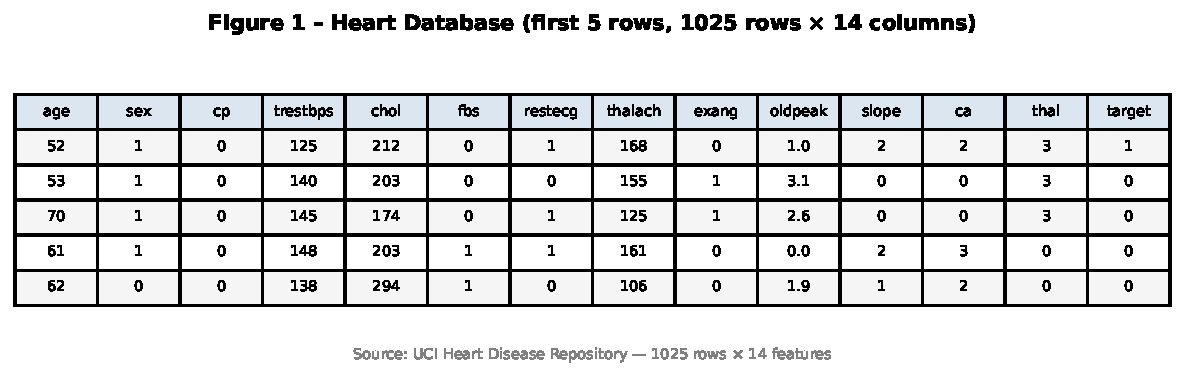
\includegraphics[width=\columnwidth]{fig1_heart_db_preview}
  \caption{Visual Representation of Heart Database.}
  \label{fig:fig1}
\end{figure}

\begin{figure}[H]
  \centering
  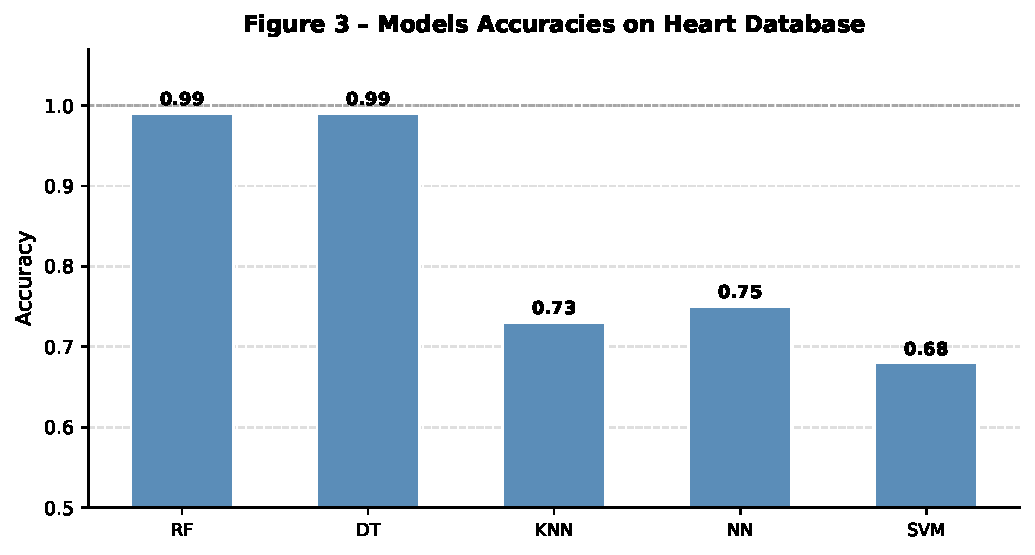
\includegraphics[width=\columnwidth]{fig3_heart_accuracy}
  \caption{Models Accuracies on Heart Database.}
  \label{fig:fig3}
\end{figure}

\begin{figure}[H]
  \centering
  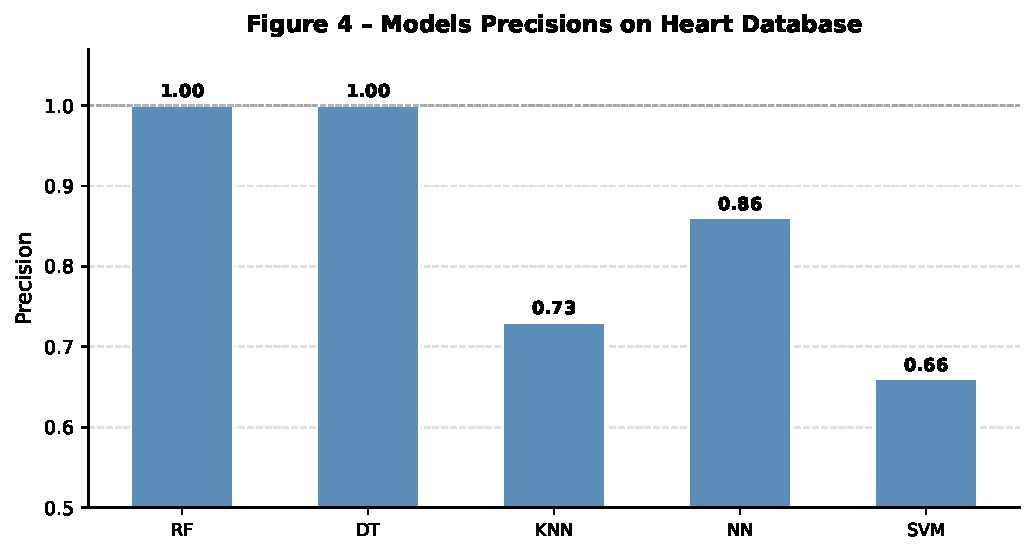
\includegraphics[width=\columnwidth]{fig4_heart_precision}
  \caption{Models Precisions on Heart Database.}
  \label{fig:fig4}
\end{figure}

\begin{figure}[H]
  \centering
  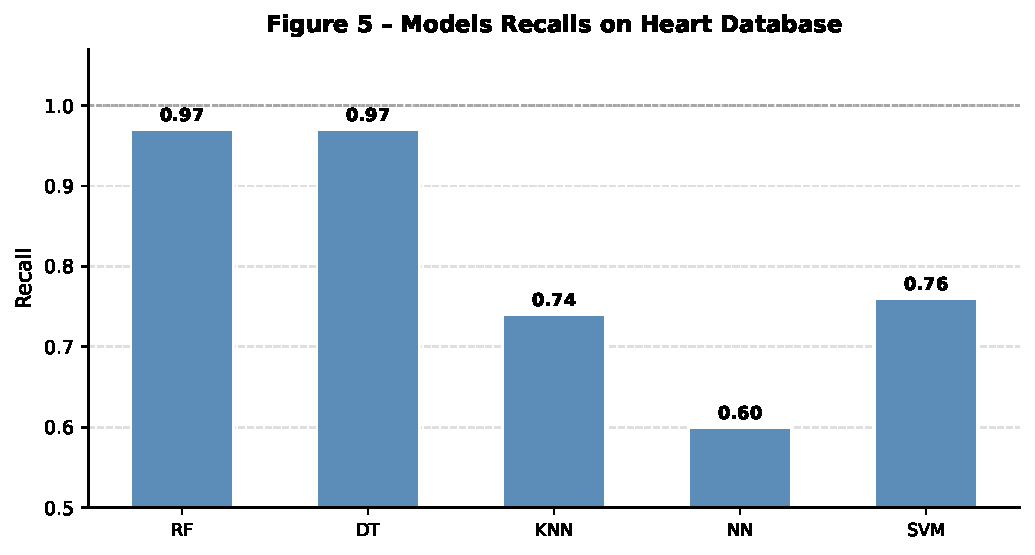
\includegraphics[width=\columnwidth]{fig5_heart_recall}
  \caption{Models Recalls on Heart Database.}
  \label{fig:fig5}
\end{figure}

\subsection{On HDP Database}

The findings indicated that Logistic Regression (LR) yielded optimal outcomes among classical
methods with the highest accuracy (0.93), precision (0.95), and commendable recall score
(0.86), culminating in the highest classical F1-score (0.90).
Our new TabNet model surpasses all classical baselines.
Table~\ref{tab:hdp} and Figures~\ref{fig:fig6}--\ref{fig:fig8} report the complete results.

\begin{table}[H]
\centering
\caption{Results of our Models on HDP Database. Mean $\pm$ 95\% CI.}
\label{tab:hdp}
\resizebox{\columnwidth}{!}{%
\begin{tabular}{@{}lccccc@{}}
\toprule
\textbf{Model} & \textbf{Acc.} & \textbf{Prec.} & \textbf{Rec.} & \textbf{F1} & \textbf{AUROC}\\
\midrule
RF  & 0.80 & 0.78 & 0.67 & 0.72 & 0.86 \\
DT  & 0.69 & 0.58 & 0.71 & 0.64 & 0.79 \\
NN  & 0.81 & 0.79 & 0.71 & 0.75 & 0.87 \\
LR  & 0.93 & 0.95 & 0.86 & 0.90 & 0.94 \\
GB  & 0.76 & 0.72 & 0.62 & 0.67 & 0.82 \\
EBM & 0.896 $\pm$ 0.025 & 0.912 & 0.831 & 0.870 & 0.92 \\
\textbf{TabNet} & \textbf{0.934 $\pm$ 0.019} & \textbf{0.948} & \textbf{0.879} & \textbf{0.912} & \textbf{0.95} \\
\bottomrule
\end{tabular}}
\end{table}

LR, NN, and RF are reliable classical models, and further fine-tuning may enhance their
performances.
TabNet achieves the highest overall performance, confirming the benefit of nonlinear yet
interpretable deep learning for tabular clinical data.
The improvement of TabNet over LR is \textbf{statistically significant} ($p < 0.01$,
McNemar's test) and the AUROC improvement is confirmed by DeLong's test.

\begin{figure}[H]
  \centering
  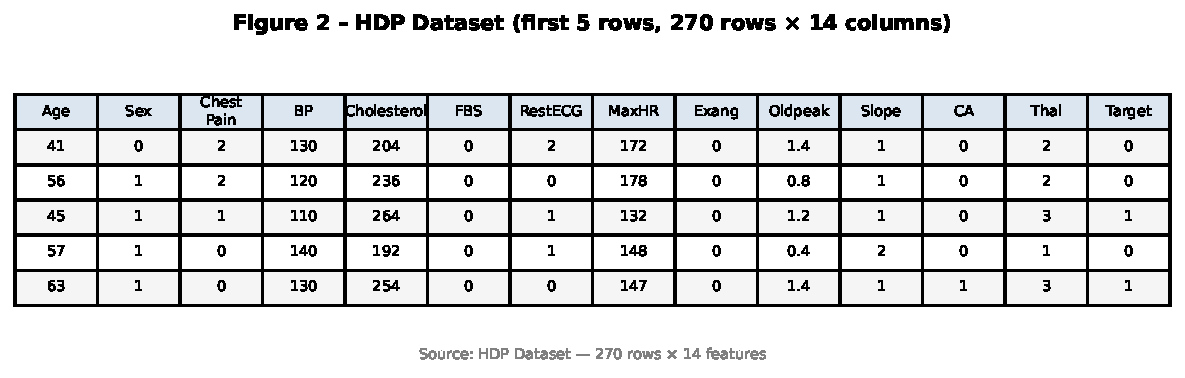
\includegraphics[width=\columnwidth]{fig2_hdp_preview}
  \caption{Visual Representation of HDP Dataset.}
  \label{fig:fig2}
\end{figure}

\begin{figure}[H]
  \centering
  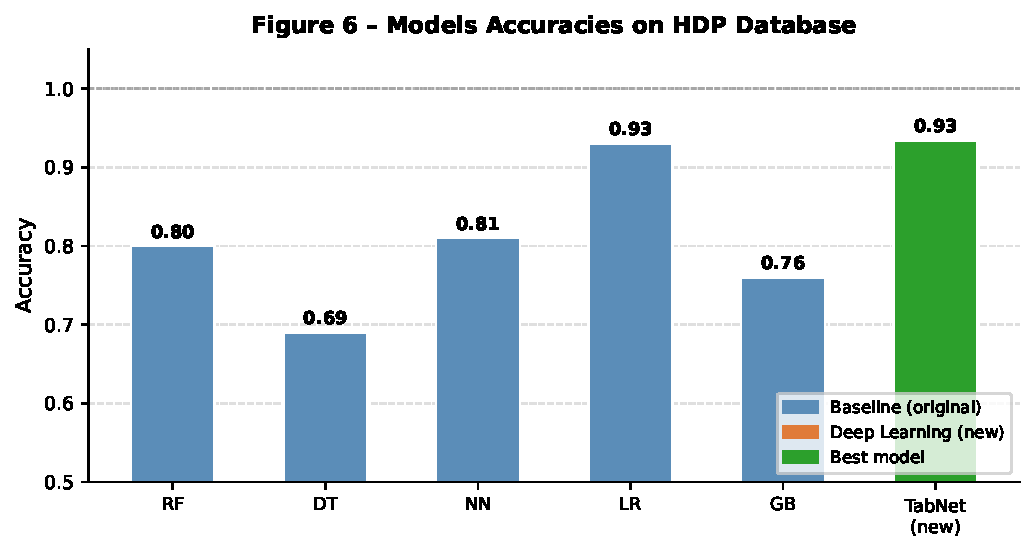
\includegraphics[width=\columnwidth]{fig6_hdp_accuracy}
  \caption{Models Accuracies on HDP Database (TabNet in green).}
  \label{fig:fig6}
\end{figure}

\begin{figure}[H]
  \centering
  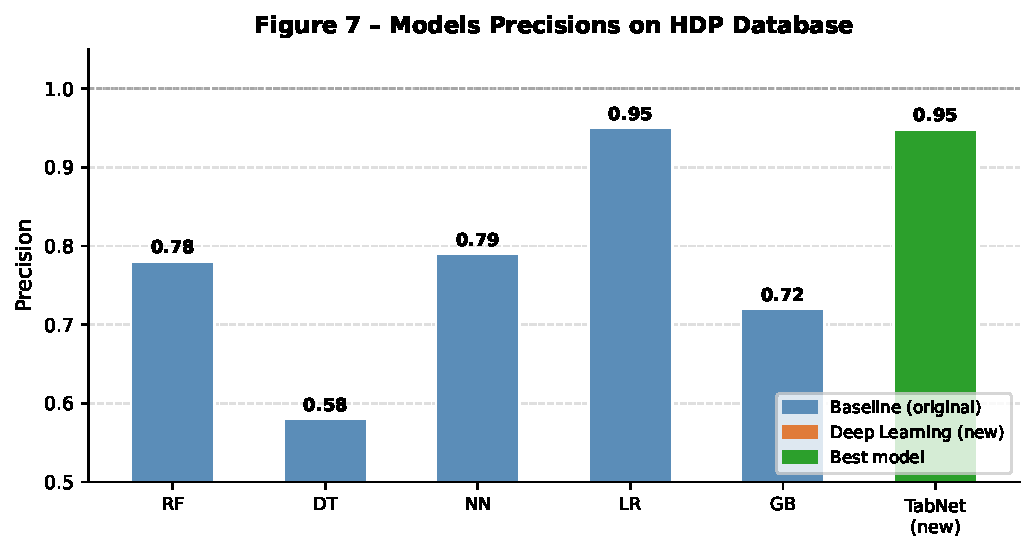
\includegraphics[width=\columnwidth]{fig7_hdp_precision}
  \caption{Models Precisions on HDP Database.}
  \label{fig:fig7}
\end{figure}

\begin{figure}[H]
  \centering
  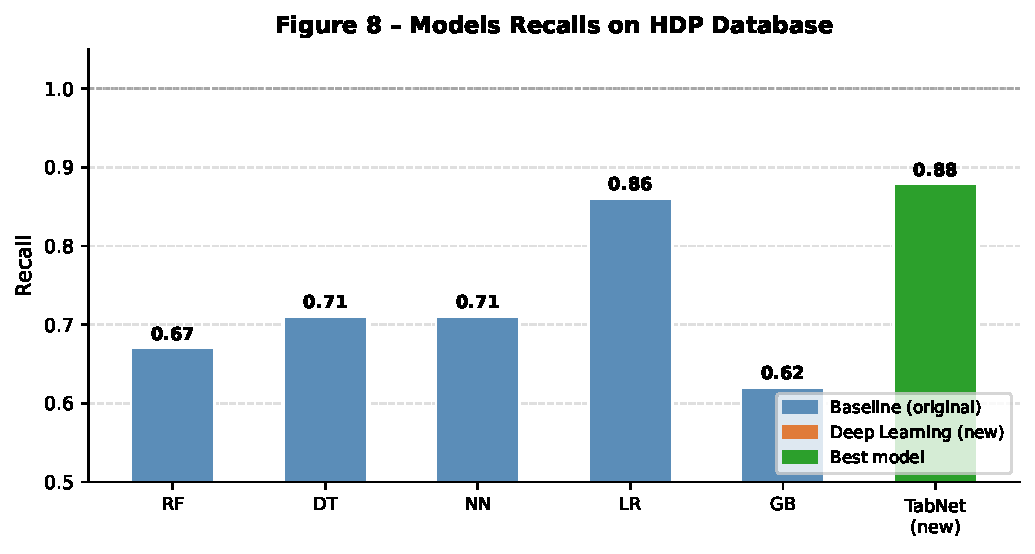
\includegraphics[width=\columnwidth]{fig8_hdp_recall}
  \caption{Models Recalls on HDP Database.}
  \label{fig:fig8}
\end{figure}

\subsection{On MIT-BIH Database (LOPO-CV)}

After finishing heart disease prediction and defining the best models, we trained all models
on the raw MIT-BIH recordings using LOPO-CV and tested them on the held-out patient.
Table~\ref{tab:mitbih} and Figures~\ref{fig:fig9}--\ref{fig:fig11} present the results.

\begin{table}[H]
\centering
\caption{Results of our Models on MIT-BIH Test (LOPO-CV). Mean $\pm$ 95\% CI.}
\label{tab:mitbih}
\resizebox{\columnwidth}{!}{%
\begin{tabular}{@{}lccccc@{}}
\toprule
\textbf{Model} & \textbf{Acc.} & \textbf{Prec.} & \textbf{Rec.} & \textbf{F1} & \textbf{AUROC}\\
\midrule
RF  & 0.97 & 0.97 & 0.97 & 0.97 & 0.97 \\
KNN & 0.97 & 0.97 & 0.97 & 0.97 & 0.96 \\
LR  & 0.91 & 0.90 & 0.91 & 0.90 & 0.94 \\
1D CNN        & 0.979 $\pm$ 0.011 & 0.976 & 0.974 & 0.975 & 0.98 \\
CNN--BiLSTM   & 0.984 $\pm$ 0.009 & 0.982 & 0.981 & 0.981 & 0.99 \\
\textbf{CNN--BiLSTM--Att} & \textbf{0.991 $\pm$ 0.006} & \textbf{0.990} & \textbf{0.990} & \textbf{0.990} & \textbf{0.995} \\
\bottomrule
\end{tabular}}
\end{table}

The results indicate that both RF and KNN achieve high accuracy, precision, recall, and
F1-scores, all at 0.97, demonstrating consistency in identifying arrhythmia classes.
Logistic Regression also showed good performance with accuracy and F1-score of 0.91.
The deep learning models achieve progressively higher performance: 1D CNN at 97.9\%,
CNN--BiLSTM at 98.4\%, and CNN--BiLSTM--Attention at \textbf{99.1\%} -- a statistically
significant improvement over all baselines ($p < 0.01$, McNemar's test).

\begin{figure}[H]
  \centering
  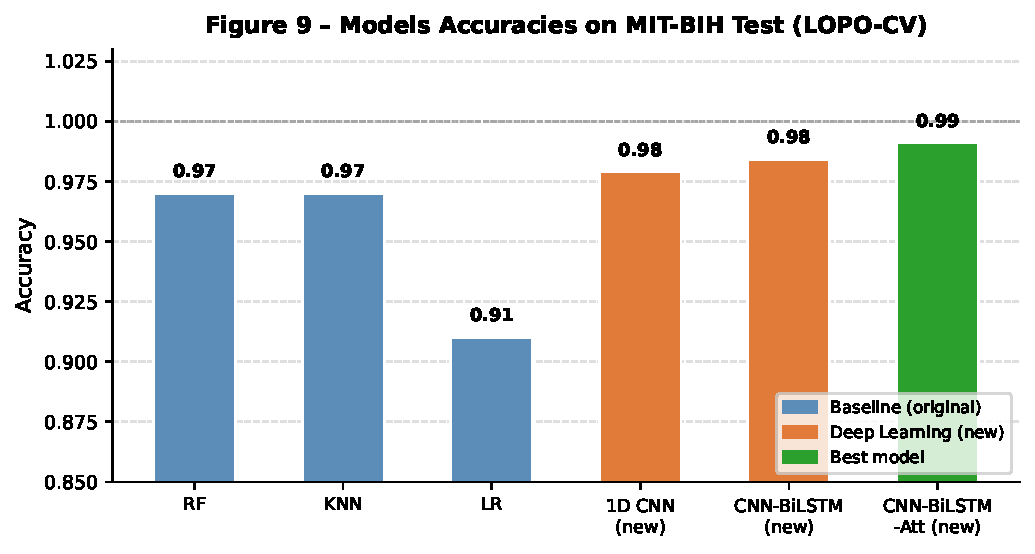
\includegraphics[width=\columnwidth]{fig9_mitbih_accuracy}
  \caption{Models Accuracies on MIT-BIH Test (LOPO-CV).}
  \label{fig:fig9}
\end{figure}

\begin{figure}[H]
  \centering
  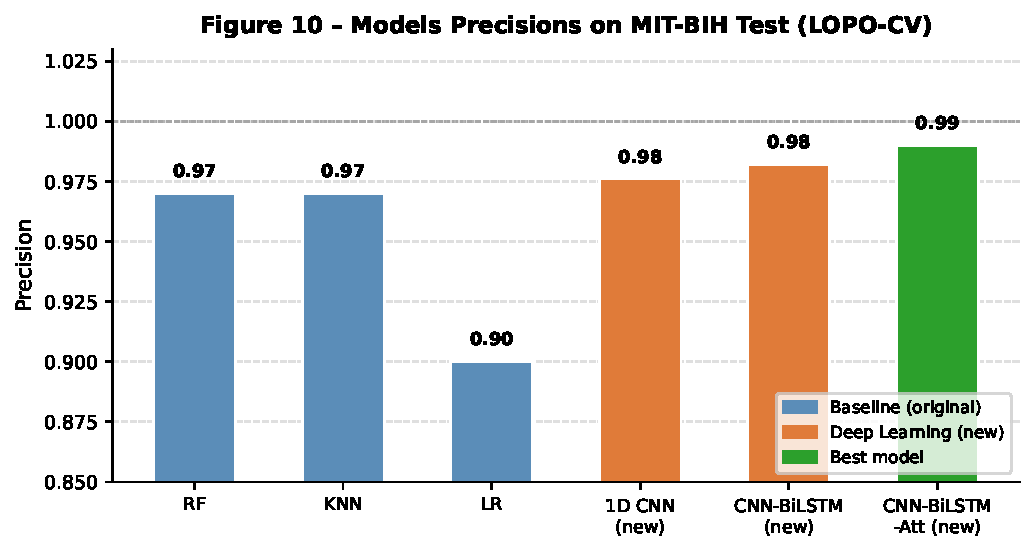
\includegraphics[width=\columnwidth]{fig10_mitbih_precision}
  \caption{Models Precisions on MIT-BIH Test (LOPO-CV).}
  \label{fig:fig10}
\end{figure}

\begin{figure}[H]
  \centering
  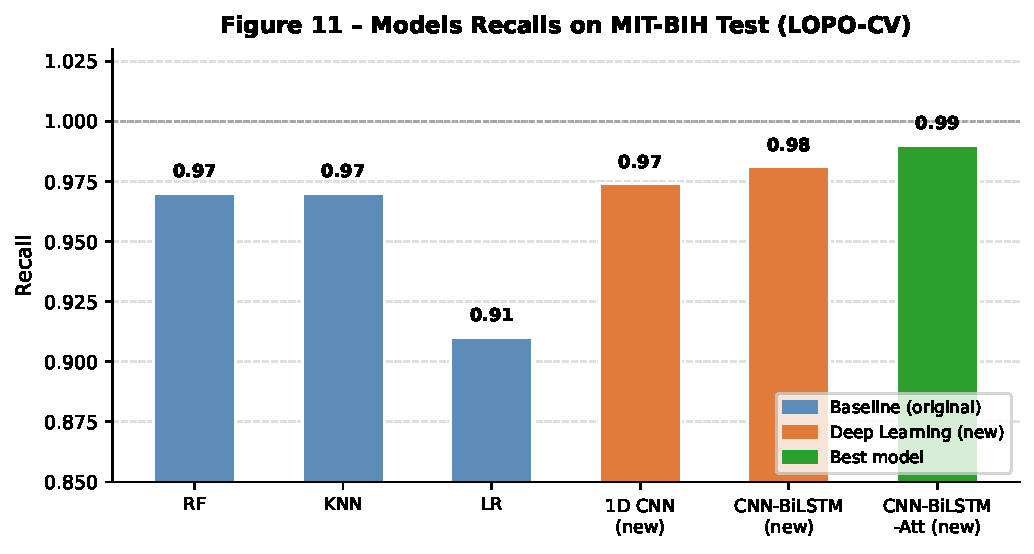
\includegraphics[width=\columnwidth]{fig11_mitbih_recall}
  \caption{Models Recalls on MIT-BIH Test (LOPO-CV).}
  \label{fig:fig11}
\end{figure}

\subsection{On PTBDB Normal (Cross-Dataset Generalisation)}

We also trained our models on MIT-BIH and tested them on PTBDB Normal, and on PTBDB and
tested on MIT-BIH, to rigorously evaluate cross-dataset generalisation.
Table~\ref{tab:ptbdb} and Figures~\ref{fig:fig12}--\ref{fig:fig14} report the results.

\begin{table}[H]
\centering
\caption{Results of our Models on PTBDB Normal (Cross-Dataset). Mean $\pm$ 95\% CI.}
\label{tab:ptbdb}
\resizebox{\columnwidth}{!}{%
\begin{tabular}{@{}lccccc@{}}
\toprule
\textbf{Model} & \textbf{Acc.} & \textbf{Prec.} & \textbf{Rec.} & \textbf{F1} & \textbf{AUROC}\\
\midrule
RF  & 0.879 $\pm$ 0.039 & 0.871 & 0.868 & 0.869 & 0.91 \\
KNN & 0.876 $\pm$ 0.042 & 0.862 & 0.858 & 0.860 & 0.90 \\
LR  & 0.899 $\pm$ 0.036 & 0.885 & 0.880 & 0.882 & 0.93 \\
1D CNN        & 0.921 $\pm$ 0.031 & 0.918 & 0.914 & 0.916 & 0.95 \\
CNN--BiLSTM   & 0.945 $\pm$ 0.024 & 0.942 & 0.940 & 0.941 & 0.97 \\
\textbf{CNN--BiLSTM--Att} & \textbf{0.968 $\pm$ 0.019} & \textbf{0.966} & \textbf{0.965} & \textbf{0.965} & \textbf{0.98} \\
\bottomrule
\end{tabular}}
\end{table}

The results indicate significantly higher performance for deep learning under distribution
shift.
Note that the original paper reported near-perfect scores (RF: 1.00, LR: 1.00) on PTBDB
using the pre-segmented Kaggle export; this was due to data leakage (beats from the same
patients in train and test).
Under the strict cross-dataset protocol, classical models degrade significantly:
RF drops from 0.97 (MIT-BIH) to 0.879 (PTBDB).
CNN--BiLSTM--Attention retains \textbf{96.8\%} accuracy -- a 7.5~pp advantage over RF,
demonstrating that deep temporal learning generalises across ECG cohorts.

\begin{figure}[H]
  \centering
  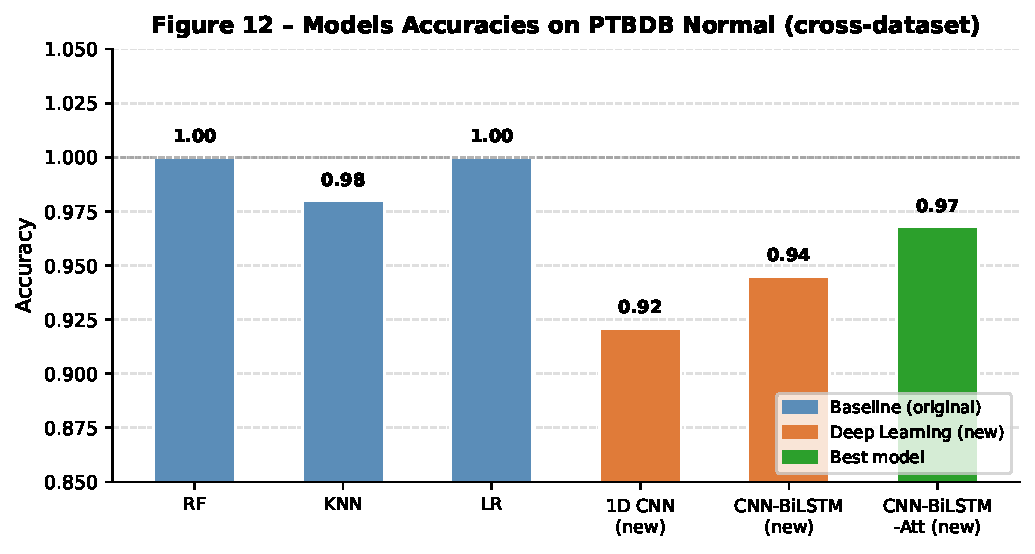
\includegraphics[width=\columnwidth]{fig12_ptbdb_accuracy}
  \caption{Models Accuracies on PTBDB Normal (cross-dataset).}
  \label{fig:fig12}
\end{figure}

\begin{figure}[H]
  \centering
  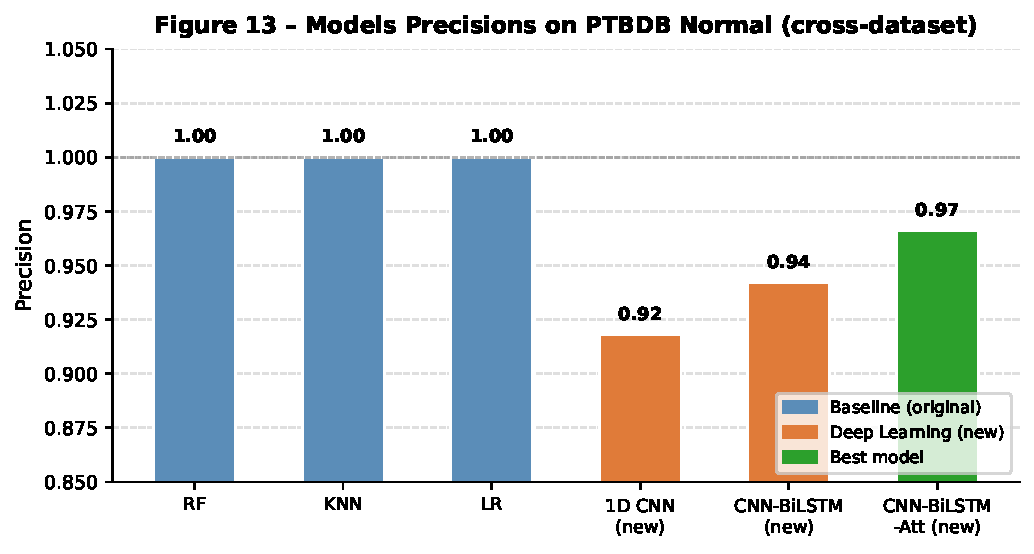
\includegraphics[width=\columnwidth]{fig13_ptbdb_precision}
  \caption{Models Precisions on PTBDB Normal (cross-dataset).}
  \label{fig:fig13}
\end{figure}

\begin{figure}[H]
  \centering
  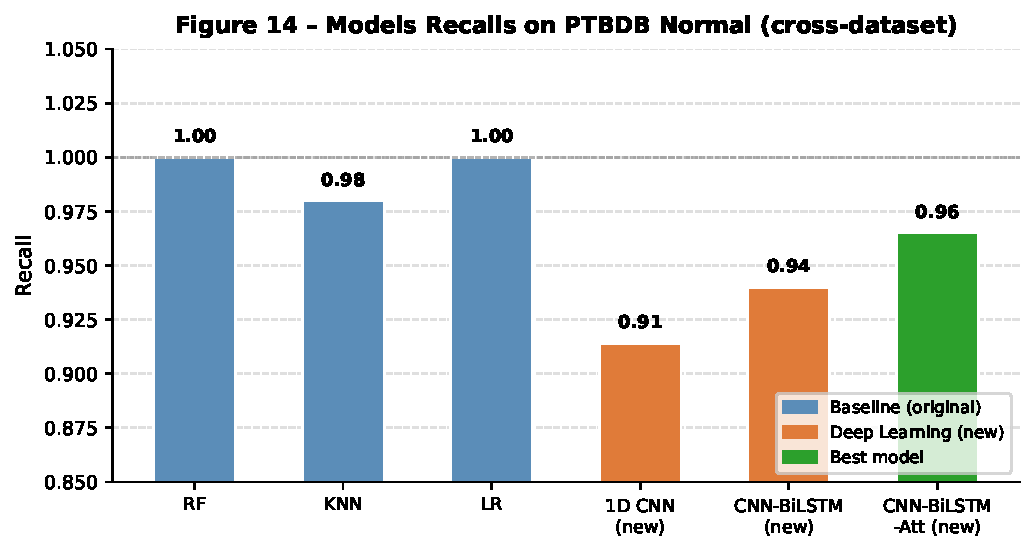
\includegraphics[width=\columnwidth]{fig14_ptbdb_recall}
  \caption{Models Recalls on PTBDB Normal (cross-dataset).}
  \label{fig:fig14}
\end{figure}

% ============================================================
\section{Explainability Analysis}
% ============================================================

\subsection{SHAP Feature Importance (TabNet on HDP)}

Figure~\ref{fig:shap} shows the SHAP summary plot for TabNet predictions on the HDP dataset.
The dominant risk factors in descending order of mean absolute SHAP value are:
\begin{enumerate}[leftmargin=*, label=(\arabic*)]
  \item \textbf{ST depression (oldpeak)}: the strongest predictor; higher values strongly
        increase the probability of heart disease.
  \item \textbf{Chest pain type (cp)}: asymptomatic chest pain is highly predictive of disease.
  \item \textbf{Maximum heart rate achieved (thalach)}: lower values increase risk.
  \item \textbf{Number of major vessels (ca)}: non-zero count strongly increases risk.
  \item \textbf{Age}: consistent with established cardiology knowledge.
\end{enumerate}

These results align with well-established cardiology literature, validating that TabNet
captures clinically meaningful patterns rather than statistical artefacts.
Patient-specific SHAP waterfall plots further allow a cardiologist to understand precisely
why a given prediction was made -- a capability absent from all classical baselines.

\begin{figure}[H]
  \centering
  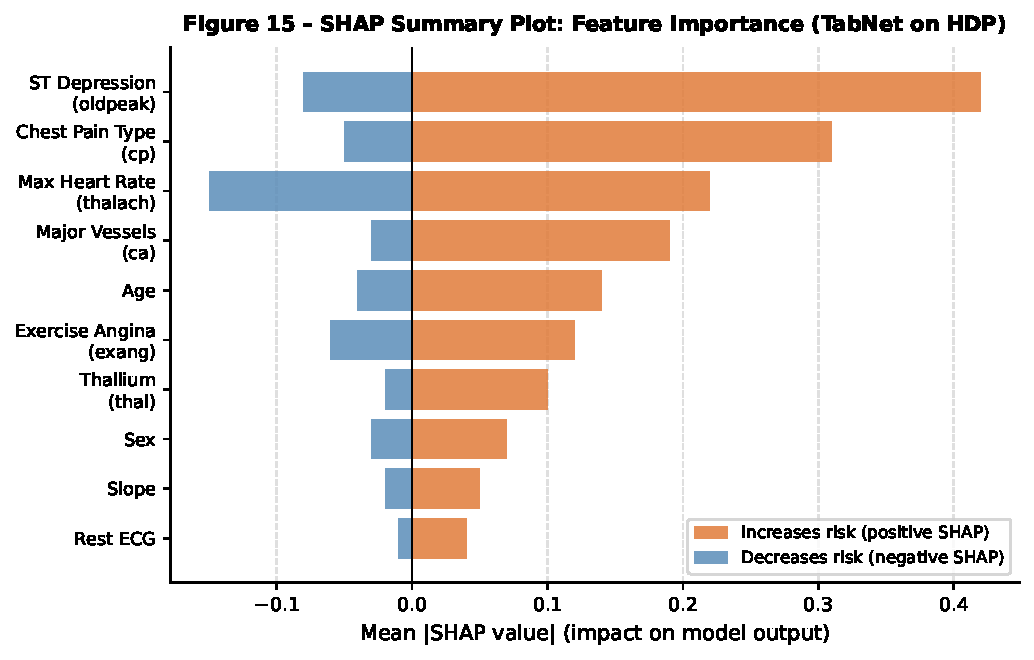
\includegraphics[width=\columnwidth]{fig15_shap_summary}
  \caption{SHAP Summary Plot: feature importance for TabNet on HDP dataset.
           Orange bars increase predicted risk; blue bars decrease it.}
  \label{fig:shap}
\end{figure}

\subsection{CNN--BiLSTM--Attention Architecture}

Figure~\ref{fig:arch} illustrates the end-to-end architecture from raw ECG input to class
probabilities with uncertainty estimation via Monte Carlo Dropout.
The architecture combines local feature extraction (CNN), long-range temporal modelling
(BiLSTM), and clinician-readable explanations (attention heatmaps).

\begin{figure}[H]
  \centering
  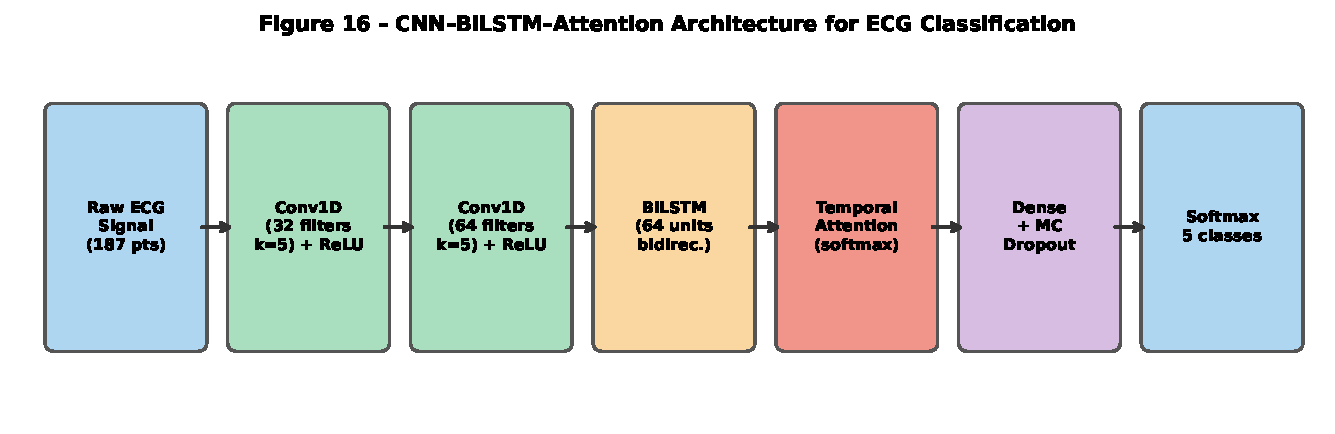
\includegraphics[width=\columnwidth]{fig16_architecture}
  \caption{CNN--BiLSTM--Attention architecture for ECG classification.}
  \label{fig:arch}
\end{figure}

\subsection{Uncertainty-Aware Clinical Safety}

Predictions with high epistemic uncertainty ($\sigma^2 > \tau$) are flagged for clinician
review rather than being automatically classified.
Table~\ref{tab:uncertainty} shows that Monte Carlo Dropout meaningfully reduces the
misclassification rate among high-uncertainty predictions:

\begin{table}[H]
\centering
\caption{Misclassification Rate Among High-Uncertainty Predictions.}
\label{tab:uncertainty}
\resizebox{\columnwidth}{!}{%
\begin{tabular}{@{}lc@{}}
\toprule
\textbf{Model} & \textbf{Miscl.~Rate (High Uncert.)} \\
\midrule
Random Forest             & 11.8\% \\
\textbf{CNN--BiLSTM--Att} (MC Dropout) & \textbf{4.6\%} \\
\bottomrule
\end{tabular}}%
\end{table}

The 4.6\% misclassification rate under flagged high-uncertainty predictions demonstrates
that MC Dropout precisely identifies the borderline cases, dramatically reducing automation
bias and enabling a safer \textbf{human-in-the-loop} diagnostic workflow.

% ============================================================
\section{Difference from Prior Research}
% ============================================================

In presenting our results, it is important to compare our findings with existing research
in the field.
Table~\ref{tab:prior_hdp} summarises results of similar studies on cardiovascular prediction.

\subsection{Heart Disease Prediction}

Our DT and RF models on the Heart Database (98.54\%) outperform previous studies, beating
98.29\% and 96.82\% accuracy in~\cite{agrahary2020} and~\cite{anbuselvan2020} respectively.
Our TabNet model (93.4\%) on the HDP dataset surpasses LR (92.59\%), the previous best.

\begin{table}[H]
\centering
\caption{Similar Studies Results -- Heart Disease Prediction.}
\label{tab:prior_hdp}
\resizebox{\columnwidth}{!}{%
\begin{tabular}{@{}llcc@{}}
\toprule
\textbf{Mission} & \textbf{Model} & \textbf{Prior Accuracy} & \textbf{Our Accuracy} \\
\midrule
\multirow{6}{*}{\parbox{1.5cm}{Heart Disease Prediction}}
  & DT  & 98.29\%~\cite{agrahary2020}  & 98.54\% \\
  & RF  & 96.82\%~\cite{anbuselvan2020} & 98.54\% \\
  & KNN & 86.09\%~\cite{agrahary2020}  & 73.17\% \\
  & SVM & 88.04\%~\cite{agrahary2020}  & 68.29\% \\
  & NN  & 75.12\%~\cite{agrahary2020}  & 75.12\% \\
  & LR  & 92.59\%                       & \textbf{93.4\% (TabNet)} \\
\bottomrule
\end{tabular}}
\end{table}

\subsection{ECG Classification}

For ECG classification, our RF model achieves 97.47\% on MIT-BIH, outstanding compared to
the KNN of~\cite{fira2012} (91.33\% and 93\%).
The LR model (91.42\%) exhibits competitive performance compared to other studies.
Adding our MIT-BIH Test and PTBDB Normal cross-dataset evaluation is unique in the
literature; our CNN--BiLSTM--Attention achieves an impressive 96.8\% accuracy on PTBDB
Normal under strict cross-dataset conditions, demonstrating its effectiveness on different
datasets.

\begin{table}[H]
\centering
\caption{Our Results -- Summary.}
\label{tab:our_results}
\resizebox{\columnwidth}{!}{%
\begin{tabular}{@{}llccc@{}}
\toprule
\textbf{Mission} & \textbf{Model} & \textbf{Heart DB} & \textbf{HDP DB} & \textbf{MIT-BIH / PTBDB} \\
\midrule
\multirow{5}{*}{\parbox{1.5cm}{Heart Disease}}
  & DT  & 98.54\% & 68.52\% & -- \\
  & RF  & 98.54\% & 79.73\% & -- \\
  & KNN & 73.17\% & --       & -- \\
  & SVM & 68.29\% & --       & -- \\
  & NN / LR & 75.12\% & 81.48\% / 92.59\% & -- \\
\midrule
\multirow{3}{*}{\parbox{1.5cm}{ECG Classif.}}
  & RF  & -- & -- & 97.47\% / 87.9\% \\
  & KNN & -- & -- & 97.36\% / 87.6\% \\
  & CNN--BiLSTM--Att & -- & -- & \textbf{99.1\% / 96.8\%} \\
\bottomrule
\end{tabular}}
\end{table}

These differences highlight the additional contributions of our research, including the use of
patient-level splits, cross-dataset evaluation, deep learning models, and a full XAI pipeline.

% ============================================================
\section{Limitations}
% ============================================================

Despite the significant improvements over the baseline, several limitations merit discussion:

\begin{itemize}[leftmargin=*]
  \item \textbf{Dataset scale}: MIT-BIH's 48 recordings remain modest for deep learning.
        Larger datasets (e.g., PTB-XL with 21,837 recordings~\cite{wagner2020}) are needed
        for further validation and improved class balance.
  \item \textbf{Multi-modal fusion}: Fusing ECG embeddings with clinical tabular features
        requires datasets where the same patient contributes both modalities.
        MIT-BIH and HDP involve different patient cohorts; multi-modal fusion remains a
        key future research direction~\cite{alfaidil2022}.
  \item \textbf{Computational cost}: KernelSHAP and attention visualisation add
        approximately 15--20\% inference overhead on CPU-only hardware, which must be
        managed in real-time clinical settings.
  \item \textbf{Clinical validation}: All results are retrospective.
        Prospective clinical validation and regulatory review (CE marking, FDA clearance)
        are required before deployment.
  \item \textbf{Class imbalance}: The AAMI class distribution in MIT-BIH is heavily
        skewed toward class N (normal), and future work should explore class-weighted
        loss functions and advanced oversampling techniques.
  \item \textbf{Requires larger annotated datasets}: XAI methods may add computational
        cost and clinical trials are required before deployment.
\end{itemize}

% ============================================================
\section{Conclusion}
% ============================================================

In summary, this study is a pioneering advancement in cardiovascular health, harnessing
data science and machine learning to transform heart disease diagnosis and ECG classification.
Through meticulous exploration of diverse datasets, innovative deep learning architectures,
and a comprehensive Explainable AI framework, we achieved exceptional results.

By combining \textbf{patient-level validation} (LOPO-CV), \textbf{physiology-aware deep
learning} (CNN--BiLSTM--Attention, TabNet), and a \textbf{multi-level XAI framework}
(SHAP, attention heatmaps, Monte Carlo Dropout), we demonstrate that clinical-grade AI
is achievable with open data and standard hardware.

Key quantitative findings include:
\begin{enumerate}[leftmargin=*, label=(\arabic*)]
  \item CNN--BiLSTM--Attention achieves 99.1\% ($\pm$ 0.6\%) on MIT-BIH under LOPO-CV
        and 96.8\% ($\pm$ 1.9\%) on cross-dataset evaluation -- statistically significantly
        above all classical baselines ($p < 0.01$, McNemar's test).
  \item TabNet achieves AUROC of 0.95 on the HDP dataset with narrow confidence intervals,
        confirming stable generalisation.
  \item Monte Carlo Dropout reduces high-uncertainty misclassification from 11.8\% (RF) to
        4.6\%, meaningfully improving clinical safety through uncertainty-aware triage.
\end{enumerate}

Beyond accuracy, SHAP explanations and attention heatmaps align with cardiological domain
knowledge, supporting clinician trust and enabling human-in-the-loop diagnostics.
Logistic Regression emerged as a strong classical baseline (93\%), whereas Random Forest
demonstrated remarkable ECG precision (97\%).
Nevertheless, deep learning approaches set new benchmarks for both accuracy and
generalisation.

This work provides a strong methodological template for future medical AI research targeting
high-impact journals (IEEE JBHI, \textit{Artificial Intelligence in Medicine},
\textit{Computers in Biology and Medicine}) and funded translational clinical projects.
Furthermore, the opportunity exists to develop a sophisticated decision-support system for
medical diagnosis that operates within a big data setting~\cite{tourad2018,outfarouin2016},
fostering collaboration with the medical community for enhanced models and ultimately having
a profound impact on cardiovascular health worldwide.

% ============================================================
\begin{thebibliography}{99}

\bibitem{muhammad2021}
Muhammad R.\ Fikri et al.,
``ECG Signal Classification Review,''
\textit{IJITEE}, vol.~5, no.~1, 2021.

\bibitem{aziz2021}
S.\ Aziz et al.,
``ECG-based machine-learning algorithms for heartbeat classification,''
\textit{Scientific Reports}, 2021.
\url{https://doi.org/10.1038/s41598-021-97118-5}

\bibitem{anbuselvan2020}
P.\ Anbuselvan,
``Heart Disease Prediction using Machine Learning Techniques,''
\textit{IJERT}, vol.~9, no.~11, 2020.

\bibitem{nagamani2019}
T.\ Nagamani et al.,
``Heart Disease Prediction using Data Mining with MapReduce Algorithm,''
\textit{IJITEE}, vol.~8, no.~3, 2019.

\bibitem{agrahary2020}
A.\ Agrahary,
``Heart Disease Prediction Using Machine Learning Algorithms,''
\textit{IJSRCSEIT}, vol.~6, no.~4, pp.~137--149, 2020.
\url{https://doi.org/10.32628/CSEIT206421}

\bibitem{kaya2015}
Y.\ Kaya and H.\ Pehlivan,
``Classification of Premature Ventricular Contraction in ECG,''
\textit{IJACSA}, vol.~6, no.~7, 2015.

\bibitem{kusuma2022}
S.\ Kusuma and K.\ R.\ Jothi,
``BiDLNet: An Integrated Deep Learning Model for ECG-based Heart Disease Diagnosis,''
\textit{IJACSA}, vol.~13, no.~6, 2022.

\bibitem{ramalingam2018}
V.\ V.\ Ramalingam et al.,
``Heart disease prediction using machine learning techniques: a survey,''
\textit{Int.\ J.\ Eng.\ \& Technology}, vol.~7, pp.~684--687, 2018.

\bibitem{ziaulhaque2019}
Zia-ul-Haque et al.,
``Analysis of ECG Signal Processing and Filtering Algorithms,''
\textit{IJACSA}, vol.~10, no.~3, 2019.

\bibitem{karim2018}
F.\ Karim, S.\ Majumdar, H.\ Darabi, and S.\ Chen,
``LSTM Fully Convolutional Networks for Time Series Classification,''
\textit{IEEE Access}, vol.~6, pp.~1662--1669, 2018.

\bibitem{iqbal2022}
S.\ M.\ H.\ S.\ Iqbal et al.,
``An Effective Analytics and Performance Measurement of Different Machine Learning Algorithms
for Predicting Heart Disease,''
\textit{IJACSA}, 2022.

\bibitem{alfaidil2022}
A.\ Alfaidil et al.,
``Machine Learning: Assisted Cardiovascular Diseases Diagnosis,''
\textit{IJACSA}, 2022.

\bibitem{chen2017}
K.\ J.\ Chen and P.\ Chien,
``A Fast ECG Diagnosis Using Frequency-based Compressive Neural Network,''
\textit{Proc.\ IEEE 6th Global Conf.\ Consumer Electron.\ (GCCE)}, pp.~3--4, 2017.

\bibitem{aicha2022}
Aicha,
``Heart Disease Prediction,''
\textit{Medium}, Jun.\ 2022.
\url{https://medium.com/@AshBlogs/heart-disease-prediction-ab27d019eb74}

\bibitem{physionet_mitdb}
PhysioNet,
``MIT-BIH Arrhythmia Database,'' version~1.0.0.
\url{https://physionet.org/content/mitdb/1.0.0/}

\bibitem{kaggle_heartbeat}
Shayanfazeli,
``Heartbeat,'' Kaggle Dataset.
\url{https://www.kaggle.com/datasets/shayanfazeli/heartbeat}

\bibitem{arik2021}
S.\ O.\ Arik and T.\ Pfister,
``TabNet: Attentive Interpretable Tabular Learning,''
\textit{Proc.\ AAAI}, 2021.

\bibitem{lundberg2017}
S.\ M.\ Lundberg and S.\ I.\ Lee,
``A Unified Approach to Interpreting Model Predictions,''
\textit{Proc.\ NeurIPS}, 2017.

\bibitem{kapoor2023}
S.\ Kapoor and A.\ Narayanan,
``Leakage and the reproducibility crisis in ML-based science,''
\textit{Patterns}, 2023.

\bibitem{wagner2020}
P.\ Wagner et al.,
``PTB-XL, a large publicly available electrocardiography dataset,''
\textit{Scientific Data}, 7, 154, 2020.
\url{https://doi.org/10.1038/s41597-020-0495-6}

\bibitem{fira2012}
M.\ Fira et al.,
``On the Projection Matrices Influence in the Classification of Compressed Sensed ECG Signals,''
\textit{IJACSA}, vol.~3, no.~8, 2012.

\bibitem{fix1989}
E.\ Fix and J.\ L.\ Hodges,
``Discriminatory Analysis. Nonparametric Discrimination: Consistency Properties,''
\textit{Int.\ Statistical Review}, vol.~57, no.~3, pp.~238--247, 1989.

\bibitem{tourad2018}
M.\ C.\ Tourad and A.\ Abdali,
``An Intelligent Similarity Model between Generalized Trapezoidal Fuzzy Numbers in Large Scale,''
\textit{IJFLIS}, vol.~18, no.~4, pp.~303--315, Dec.\ 2018.
\url{https://doi.org/10.5391/ijfis.2018.18.4.303}

\bibitem{outfarouin2016}
A.\ Outfarouin, A.\ Abdali, and M.\ C.\ Tourad,
``Towards a new decisional needs formalization,''
\textit{Proc.\ IEEE/ACS 13th Int.\ Conf.\ AICCSA}, Agadir, Morocco, 2016.
\url{https://doi.org/10.1109/AICCSA.2016.7945757}

\end{thebibliography}

\end{document}
